%-------------------------------------------------------
\section{The Importance of Liquidity}
%-------------------------------------------------------

\begin{frame}

\begin{center}
{\LARGE The Importance of Liquidity}
\end{center}

\end{frame}

%-------------------------------------------------------

%-------------------------------------------------------

\begin{frame}{Liquidity Crisis}

The crisis saw dramatic disruption to, and loss of, liquidity
	\begin{itemize}
	\item	Many ways to define liquidity
	\item	Ability to sell/liquidate asset rapidly at a reasonable price
	\item	Ability to borrow on reasonable terms easily / quickly
	\item	With collateralization, the two definitions are closely related
	\end{itemize}
\vspace{1.5mm}
Liquidity problems interacted with, but to an important degree, are distinct from solvency problems
	\begin{itemize}
	\item	Liquidity: Can I sell assets/borrow quickly at a `fair price'?
	\item	Solvency: Value of assets $>$ liabilities
	\end{itemize}
\vspace{1.5mm}	
Common models of banks' liquidity risk build on \href{https://www.jstor.org/stable/1837095}{Diamond-Dybvig (1983)}
	\begin{itemize}
	\item	Explains how depositors may `run' on `maturity mismatched' banks
	\item	Banks `borrow short and lend long'
	\item	Runs affected banks and shadow banks in the crisis
	\item	Not \href{https://en.wikipedia.org/wiki/Northern_Rock}{(only)} by people \href{https://www.theatlantic.com/business/archive/2016/12/its-a-wonderful-life-banking/511592/}{queuing outside banks} but also in \href{https://www.reuters.com/article/uk-shadow-banking-qa/qa-what-is-shadow-banking-and-why-does-it-matter-idUKTRE81611Q20120207}{debt markets/shadow banking}
	\end{itemize}

\end{frame}

%-------------------------------------------------------

%-------------------------------------------------------

\begin{frame}{Diamond Dybvig (1983)}

Seminal paper: insights into \textit{deep} issues with strikingly sparse model
	\begin{itemize}
	\item	Why maturity transformation by banks might be efficient
	\item	Why this phenomenon also renders them vulnerable to runs
	\item	Why a \textit{solvent} institution might fail, due to a lack of liquidity
	\item	The concept of liquidity - formulated precisely
	\item	Possible policy responses
	\end{itemize}
\vspace{2mm}
The original \href{https://ideas.repec.org/a/ucp/jpolec/v91y1983i3p401-19.html}{\emph{1983 paper}} is readable (one of the great papers)
	\begin{itemize}
	\item	A later summary paper, \href{https://www.richmondfed.org/-/media/richmondfedorg/publications/research/economic_quarterly/2007/spring/pdf/diamond.pdf}{\emph{Diamond (2007)}}, is an easier read
	\end{itemize}

\end{frame}

%-------------------------------------------------------

%-------------------------------------------------------

\begin{frame}{Diamond Dybvig (1983)}
\textbf{Banks borrow\ldots}
		\begin{itemize}
		\item	Liability from perspective of bank
		\item	Asset from perspective of `depositor'
		\item	Also applies to short term borrowing in money markets
		\end{itemize}
\vspace{1mm}		
\textbf{\ldots to fund investments in long(er) term projects}
	\begin{itemize}
	\item	`Illiquid' assets such as loans to build a factory
	\item	Early liquidation may reduce value of asset (loan)
	\end{itemize}
\vspace{4mm}
A principle function of banks is to create liquidity
	\begin{itemize}
	\item	Deposits (withdraw any time at face value) more liquid than assets
	\item	Investors who want liquidity will prefer to hold illiquid assets \emph{indirectly} - through the bank
	\item	This is great - when it works - but there is a nasty sting in the tail!
	\end{itemize}

\end{frame}

%-------------------------------------------------------

%-------------------------------------------------------

\begin{frame}{Diamond Dybvig (1983) - Setup}

\begin{itemize}
\item	One good
\item	Three dates: $t=0,1,2$
\item	Continuum (infinitely many, infinitesimally small) of agents
\item	Each agent endowed with a unit of the good at $t=0$
\item	\emph{Ex ante} the agents are identical (at $t=0$)
\item	But face idiosyncratic shock at $t=1$
	\begin{itemize}
	\item	With (independent) probability $\pi$ they need to consume at period 1
	\item	So with probability $1-\pi$ they need to consume at period 2
	\item	Think of first (`type 1') as impatient and second (`type 2') as `patient'
	\item	Perhaps better to imagine type 1 getting an unexpected cashflow need
	\end{itemize}
\item	As of period $0$ they have utility given by
\[
U = \pi u(C_{1}) + (1-\pi)u(C_{2})
\]
\item	Continuum of agents, independence and LOLN $\Rightarrow$ realized fraction of type 1 at $t=1$ is given by $\pi$
\end{itemize}

\end{frame}

%-------------------------------------------------------

%-------------------------------------------------------

\begin{frame}{Diamond Dybvig (1983) - Alternative `investments'}

Agents can store good from one period to the next without any cost
	\begin{itemize}
	\item	Think of this like sticking money under the mattress
	\end{itemize}
\vspace{2mm}
\textbf{Alternatively} they have access to a constant returns to scale (CRS) technology
	\begin{itemize}
	\item	One unit invested at $t=0 \Rightarrow$ return $R>1$ at $t=2$
	\item	Technology implies an `illiquid asset' in that investment only yields return $s<1$ if it is liquidated at $t=1$
	\item	Think of this as trying to quickly wind up a business or interrupt the building of a factory prematurely
	\end{itemize}
\end{frame}

%-------------------------------------------------------

%-------------------------------------------------------

\begin{frame}{Diamond Dybvig (1983) - Autarky}

Consider an agent (who does not yet know her type) choosing the scale of investment, I, in the CRS technology
\begin{itemize}
\item	Remainder, 1-I, will be stored
\item	There is no trade with the other agent by assumption (autarky) so it is a standalone problem
\end{itemize}

\vspace{2mm}
The concept of \href{https://en.wikipedia.org/wiki/Autarky}{autarky} comes up a lot in economics
\begin{itemize}
\item	Usually as a `bad thing' since trade is good (broadly speaking)
\item	Being `self-sufficient' is good in some contexts - but not when gains from trade are out there!
\item	Autarky is a simple benchmark to show scope for welfare improvement
\item	Often used to represent `punishment' in games (e.g. after a country defaults on debt, models assume it has to face autarky for a certain number of periods before countries/investors trade with them again)
\end{itemize}

\end{frame}

%-------------------------------------------------------

%-------------------------------------------------------

\begin{frame}{Diamond Dybvig (1983) - Autarky}

They look forward in time\ldots
\begin{itemize}
\item	If they turn out to be type 1 they will liquidate (only care about $C_{1}$)
\[
C_{1} = sI + 1- I
\]
\item	If they turn out to be type 2 they will continue project (only care about $C_{2}$)
\[
C_{2} = RI + 1- I
\]	
\item	Anticipating this, they choose $I$ to maximize
\[
\pi_{1}u(sI + 1- I) + (1-\pi_{2})u(RI + 1- I)
\]
\item	The FOC implies
\[
-\frac{1-\pi_{1}}{\pi_{1}} \frac{R-1}{s-1} = \frac{u'(C_{1})}{u'(C_{2})}
\]
\end{itemize}
	
\end{frame}

%-------------------------------------------------------

%-------------------------------------------------------

\begin{frame}{Diamond Dybvig (1983) - Autarky}

We can partially characterize the solution (even without specifying further utility function details)
	\begin{itemize}
	\item	Suppose $I = 0$, then $C_{1}=C_{2}=1$
	\item	Suppose $I = 1$, then $C_{1}=s$ and $C_{2}=R$
	\item	Suppose $I\in(0,1)$ then\ldots
		\begin{itemize}
		\item	$C_{1} = (s-1)I + 1 < 1$ (since $s<1$)
		\item	$C_{2} = (R-1)I + 1 < R - 1 + 1 = R$ (since $R>1$)
		\end{itemize}
	\end{itemize}
\vspace{2mm}
Note that $C_{1}\leq1$ and $C_{2}\leq R$ with at least one strict equality
	\begin{itemize}
	\item	The chosen $I$ is \emph{ex post} inefficient with probability $>0$
	\item	Type $1$: Wish had set $I=0$ as sticking it under the mattress for return of $1$ is better than $s$ from premature liquidation
	\item	Type 2: Wish had set $I=0$ since all savings would have earned $R$, rather than $1$ under the bed
	\item	They do this because they don't want to risk a complete mismatch of payoffs and their liquidity demands
	\end{itemize}
	
\end{frame}

%-------------------------------------------------------

%-------------------------------------------------------

\begin{frame}{Diamond Dybvig (1983) - Opening a financial market}

Is the problem solvable simply by opening a bond market?
	\begin{itemize}
	\item	Price in period 1 of a unit of good in period 2 is given by $p$
	\vspace{1mm}
	\item	Allows type 1 to have $C_{1} = pRI + 1 - I$
		\begin{itemize}
		\item	From selling $RI$ bonds (instead of liquidating long term investment)
		\item	The long term investment allows her to fulfill her commitment
		\end{itemize}
	\vspace{1mm}
	\item	Allows type 2 to have $C_{2} = RI + \frac{1-I}{p}$
		\begin{itemize}
		\item	From buying $\frac{1-I}{p}$ bonds (instead of storing the good for another period)
		\end{itemize}
	\vspace{1mm}
	\item	$C_{1}=pC_{2}$ and thus utility is $\uparrow(\downarrow)$ in $I$ if $pR>1(<1)$
		\begin{itemize}
		\item	Linearity in $I$ implies that an interior solution can only exist if $pR=1$
		\item	Using feasibility $(1-\pi_{1})C_{2} = RI \Rightarrow I = 1-\pi_{1}$
		\end{itemize}
	\vspace{1mm}
	\item	Then $(C_{1},C_{2})=(1,R)$ which is Pareto superior to the autarkic case (where $C_{1}\leq1$ and $C_{2}\leq R$ with at least one - typically both - strict)
	\end{itemize}
\vspace{2mm}
So opening a bond market has improved the situation, but is it `ideal'?

\end{frame}

%-------------------------------------------------------

%-------------------------------------------------------

\begin{frame}{Diamond Dybvig (1983) - Optimal (symmetric) allocation}

Suppose we simply ask what the `planning' optimum would be
\begin{itemize}
\item	We simply maximize $\pi_{1}u(C_{1}) + (1-\pi_{2})u(C_{2})$, subject to
	\begin{itemize}
	\item	Feasibility in period 1: $\pi_{1}C_{1} = 1 - I$
	\item	Feasibility in period 2: $(1-\pi_{1})C_{2} = RI$
	\end{itemize}
\vspace{2mm}	
\item	This is equivalent to choosing $I$ to maximize
\end{itemize}
\[
\pi u\left( \frac{1-I}{\pi_{1}} \right) + (1-\pi_{1}) u \left( \frac{R I}{1-\pi_{1}} \right)
\]
\begin{itemize}
\item This yields the FOC that optimal allocation $(C^{\ast}_{1},C^{\ast}_{2})$ must satisfy
\end{itemize}
\[
-u'(C^{\ast}_{1}) + Ru'(C^{\ast}_{2}) = 0
\]
\textbf{\href{https://en.wikipedia.org/wiki/Generic_property}{Generically} the (bond) market allocation won't satisfy this condition}
	\begin{itemize}
	\item	Need fluke $u(\cdot)$ for it to hold with $(C_{1},C_{2})=(1,R)$ (implying $I=1-\pi_{1}$)
	\end{itemize}

\end{frame}

%-------------------------------------------------------

%-------------------------------------------------------

\begin{frame}{Diamond Dybvig (1983) - Banking equilibria}

It turns out that the presence of banks can implement the optimum, as \textbf{an} equilibrium
\begin{itemize}
\item	Suppose we have a fractional reserve system
	\begin{itemize}
	\item	Not all deposits are backed by short term assets
	\end{itemize}
\item	The bank\ldots
	\begin{itemize}
	\item	Collects agents' endowments in time 0 (deposits)
	\item	Offers the depositors the right to withdraw at any time
	\item	Invests a fraction in the long-term project
	\item	Proposes a deposit contract that allocates $(C_{1}^{\ast},C_{2}^{\ast})$ in periods 1 and 2, respectively, given a unit deposit in period 0
	\end{itemize}
\end{itemize}

\end{frame}

%-------------------------------------------------------

%-------------------------------------------------------

\begin{frame}{Diamond Dybvig (1983) - Banking equilibria}

Good equilibrium
	\begin{itemize}
	\item	Suppose type 2 agent (whose beliefs matter) believes bank will satisfy its obligations in period 2
	\item	The FOC from the planning problem $\Rightarrow$ $C_{1}^{\ast}< C_{2}^{\ast}$ so sticking with the contract is preferable to withdrawing and storing
	\item	All type 1 agents will withdraw - so the bank must have $\pi_{1}C_{1}^{\ast}$ on hand
	\item	So the bank must invest only $1-\pi_{1}C_{1}^{\ast}$ in project at $t=0$
	\item	Then the bank is solvent in this equilibrium with probability $1$
	\end{itemize}

\end{frame}

%-------------------------------------------------------

%-------------------------------------------------------

\begin{frame}{Diamond Dybvig (1983) - Banking equilibria}

Bad equilibrium (bank run)
	\begin{itemize}
	\item	Suppose bank adopts the approach above but\ldots
	\item	Suppose a type 2 agent believes all other type 2 will withdraw at $t=1$
	\item	Then bank will need to liquidate all its assets at $t=1$ yielding total value $\pi_{1} C_{1}^{\ast} + (1-\pi_{1}C_{1}^{\ast})s < 1 < C_{1}^{\ast}$ ($C_{1}^{\ast}$ is the value of its liabilities)
	\item	$\Rightarrow$ insolvent and nothing will remain to pay out in period 2
	\item	So, given these beliefs, optimal for (any and all) type 2 agents to withdraw in $t=1$
	\item	Behavior confirms the belief that induced it $\Rightarrow$ an equilibrium
	\end{itemize}
\vspace{2mm}
Deposit insurance or bailing banks out can prevent this, but\ldots
	\begin{itemize}
	\item	Dulls depositors' incentive to monitor banks and - unless properly priced - subsidizes risky investments
	\item	Huge problems with moral hazard if banks anticipate bailout
	\end{itemize}

\end{frame}

%-------------------------------------------------------

%-------------------------------------------------------

\begin{frame}{Other models of liquidity crises and runs}

There are various ways of modeling runs and liquidity crunches
\begin{itemize}
\item	Other frameworks relevant to the recent crisis are those that emphasize fire-sales
\item	There can be important feedbacks from fire-sales, depressing asset prices, to weakening of banks, requiring further sales and difficulty in obtaining funding with collateralized borrowing\ldots
\end{itemize}

\end{frame}

%-------------------------------------------------------

%-------------------------------------------------------

\begin{frame}{Vicious circles in funding and asset prices}

\begin{figure}
\begin{center}

\resizebox{0.70\textwidth}{!}{%
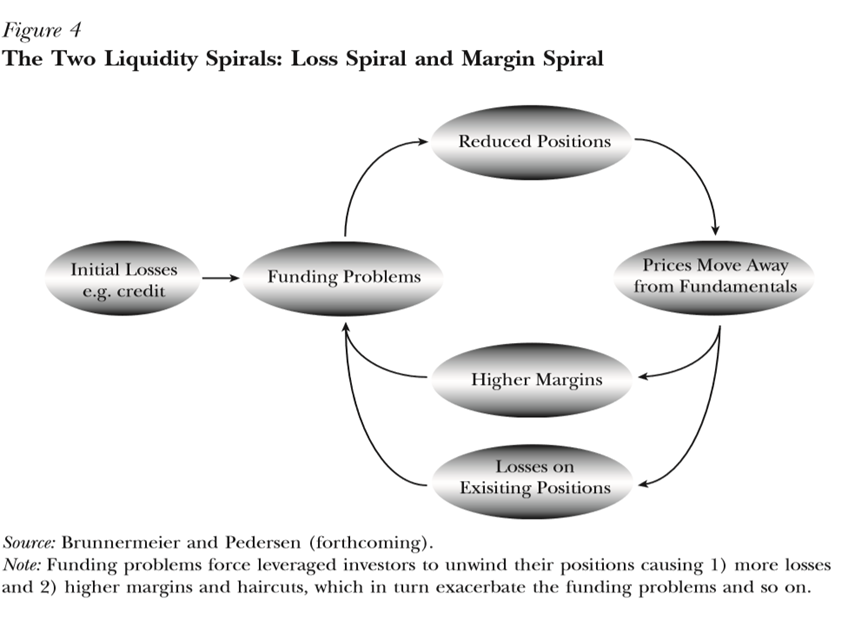
\includegraphics{Figures/liquidity_spiral.png}
}

\caption{\label{fig:L4_liquidity_spiral} Liquidity spirals feeding back into fire sales and asset price declines, feeding back into liquidity spirals\ldots. Source: \href{https://www.princeton.edu/~markus/research/papers/liquidity_credit_crunch.pdf}{Brunnermeier (2009); Bloomberg}}

\end{center}
\end{figure}

\end{frame}

